%\VignetteIndexEntry{Analyzing RNA-seq data with the "DESeq2" package}
%\VignettePackage{DESeq2}
%\VignetteEngine{knitr::knitr}

% To compile this document
% library('knitr'); rm(list=ls()); knit('DESeq2.Rnw')

\documentclass[a4paper,11pt]{article}\usepackage[]{graphicx}\usepackage[]{color}
%% maxwidth is the original width if it is less than linewidth
%% otherwise use linewidth (to make sure the graphics do not exceed the margin)
\makeatletter
\def\maxwidth{ %
  \ifdim\Gin@nat@width>\linewidth
    \linewidth
  \else
    \Gin@nat@width
  \fi
}
\makeatother

\definecolor{fgcolor}{rgb}{0.345, 0.345, 0.345}
\newcommand{\hlnum}[1]{\textcolor[rgb]{0.686,0.059,0.569}{#1}}%
\newcommand{\hlstr}[1]{\textcolor[rgb]{0.192,0.494,0.8}{#1}}%
\newcommand{\hlcom}[1]{\textcolor[rgb]{0.678,0.584,0.686}{\textit{#1}}}%
\newcommand{\hlopt}[1]{\textcolor[rgb]{0,0,0}{#1}}%
\newcommand{\hlstd}[1]{\textcolor[rgb]{0.345,0.345,0.345}{#1}}%
\newcommand{\hlkwa}[1]{\textcolor[rgb]{0.161,0.373,0.58}{\textbf{#1}}}%
\newcommand{\hlkwb}[1]{\textcolor[rgb]{0.69,0.353,0.396}{#1}}%
\newcommand{\hlkwc}[1]{\textcolor[rgb]{0.333,0.667,0.333}{#1}}%
\newcommand{\hlkwd}[1]{\textcolor[rgb]{0.737,0.353,0.396}{\textbf{#1}}}%

\usepackage{framed}
\makeatletter
\newenvironment{kframe}{%
 \def\at@end@of@kframe{}%
 \ifinner\ifhmode%
  \def\at@end@of@kframe{\end{minipage}}%
  \begin{minipage}{\columnwidth}%
 \fi\fi%
 \def\FrameCommand##1{\hskip\@totalleftmargin \hskip-\fboxsep
 \colorbox{shadecolor}{##1}\hskip-\fboxsep
     % There is no \\@totalrightmargin, so:
     \hskip-\linewidth \hskip-\@totalleftmargin \hskip\columnwidth}%
 \MakeFramed {\advance\hsize-\width
   \@totalleftmargin\z@ \linewidth\hsize
   \@setminipage}}%
 {\par\unskip\endMakeFramed%
 \at@end@of@kframe}
\makeatother

\definecolor{shadecolor}{rgb}{.97, .97, .97}
\definecolor{messagecolor}{rgb}{0, 0, 0}
\definecolor{warningcolor}{rgb}{1, 0, 1}
\definecolor{errorcolor}{rgb}{1, 0, 0}
\newenvironment{knitrout}{}{} % an empty environment to be redefined in TeX

\usepackage{alltt}
\usepackage[top=2cm,bottom=2.5cm,left=2cm,right=2cm]{geometry}

\author{M. Evers$^{1}$\\[1em]
\small{$^{1}$ The John Curtin School of Medical Research,}\\\small{The Australian National University, Canberra, Australia}}

\title{Visualisation and functional analysis of single-nucleotide modifications in mRNAs using the RNAModR package}
\IfFileExists{upquote.sty}{\usepackage{upquote}}{}
\begin{document}
\maketitle

\section{Introduction}
Following is a typical workflow for visualising and analysing single-nucleotide modifications:
\begin{enumerate}
  \item Construction of a custom transcriptome.
  \item Mapping of genome alignment-based single-nucleotide modifications to transcript coordinates.
  \item Visualisation of basic metrics, e.g. distribution of sites across different transcript sections.
  \item Enrichment analyses of single-nucleotide modifications.
\end{enumerate}
The RNAModR library is loaded following
\begin{knitrout}
\definecolor{shadecolor}{rgb}{0.969, 0.969, 0.969}\color{fgcolor}\begin{kframe}
\begin{alltt}
\hlkwd{library}\hlstd{(}\hlstr{"RNAModR"}\hlstd{)}
\end{alltt}
\end{kframe}
\end{knitrout}

\section{Reference transcriptome and transcript annotation}
RNAModR analyses the distribution of RNA modifications across mRNA transcripts and therefore requires suitable mRNA transcriptome and transcript annotation data. When RNAModR is run for the first time, a custom transcriptome is constructed based on UCSC RefSeq gene annotations and associated R data are stored locally in a single binary R file. This process can take up to 10 minutes (depending on the computer hardware), and needs to be run only once as part of a new data analysis. Subsequent re-analyses check for existing suitable transriptome data, and load the required data as part of the different anlysis routines.\par

To start our example of an analysis of the m$^{6}$A sample data \cite{Linder}, we construct the necessary transcriptome and annotation data based on the reference genome assembly version GRCh38/hg38 using
\begin{knitrout}
\definecolor{shadecolor}{rgb}{0.969, 0.969, 0.969}\color{fgcolor}\begin{kframe}
\begin{alltt}
\hlkwd{BuildTx}\hlstd{(}\hlstr{"hg38"}\hlstd{);}
\end{alltt}
\begin{verbatim}
## Found existing transcriptome data.
## To rebuild run with force = TRUE.
\end{verbatim}
\end{kframe}
\end{knitrout}

We can plot the length distribution of the different transcript sections using
\begin{knitrout}
\definecolor{shadecolor}{rgb}{0.969, 0.969, 0.969}\color{fgcolor}\begin{kframe}
\begin{alltt}
\hlkwd{LoadRefTx}\hlstd{(}\hlstr{"hg38"}\hlstd{);}
\hlkwd{PlotTxSecLength}\hlstd{(txBySec,} \hlkwc{filter} \hlstd{=} \hlkwd{c}\hlstd{(}\hlstr{"5'UTR"}\hlstd{,} \hlstr{"CDS"}\hlstd{,} \hlstr{"3'UTR"}\hlstd{,} \hlstr{"CDS_exon"}\hlstd{,} \hlstr{"Intron"}\hlstd{));}
\end{alltt}
\end{kframe}
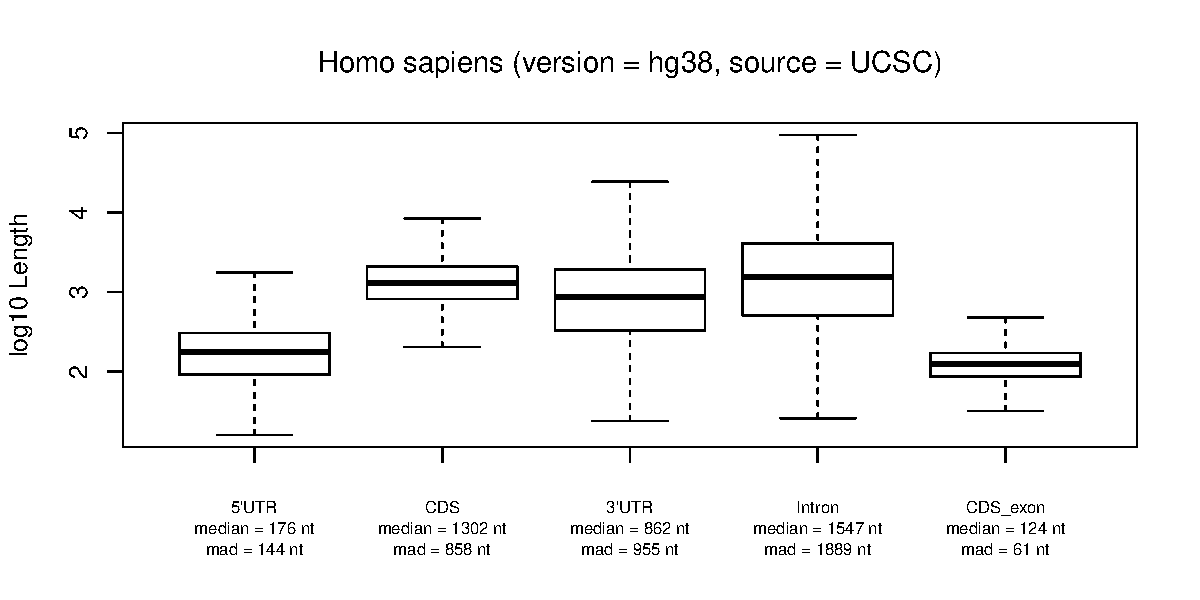
\includegraphics[width=\maxwidth]{figure/unnamed-chunk-3-1} 

\end{knitrout}

\section{Mapping RNA modifications to transcript coordinates}
Next we load a BED file containing genome locations of m$^{6}$A modifications from \cite{?}:
\begin{knitrout}
\definecolor{shadecolor}{rgb}{0.969, 0.969, 0.969}\color{fgcolor}\begin{kframe}
\begin{alltt}
\hlstd{bedFile} \hlkwb{<-} \hlkwd{system.file}\hlstd{(}\hlstr{"extdata"}\hlstd{,}
                       \hlstr{"miCLIP_m6A_Linder2015_hg38.bed"}\hlstd{,}
                       \hlkwc{package} \hlstd{=} \hlstr{"RNAModR"}\hlstd{);}
\hlstd{sites} \hlkwb{<-} \hlkwd{ReadBED}\hlstd{(bedFile);}
\hlkwd{class}\hlstd{(sites);}
\end{alltt}
\begin{verbatim}
## [1] "GRanges"
## attr(,"package")
## [1] "GenomicRanges"
\end{verbatim}
\begin{alltt}
\hlkwd{length}\hlstd{(sites);}
\end{alltt}
\begin{verbatim}
## [1] 15167
\end{verbatim}
\end{kframe}
\end{knitrout}

We map genome coordinates of the 15167 sites to the transcriptome:
\begin{knitrout}
\definecolor{shadecolor}{rgb}{0.969, 0.969, 0.969}\color{fgcolor}\begin{kframe}
\begin{alltt}
\hlstd{posSites} \hlkwb{<-} \hlkwd{SmartMap}\hlstd{(sites,} \hlkwc{id} \hlstd{=} \hlstr{"m6A"}\hlstd{,} \hlkwc{refGenome} \hlstd{=} \hlstr{"hg38"}\hlstd{);}
\end{alltt}
\end{kframe}
\end{knitrout}
The return object is an RNAModR-specific object of type txLoc, that contains a list of sites with positions within any of the transcript sections (promoter, 5'UTR, CDS, 3'UTR, intron).

We can access a txLoc to get a brief summary of the mapped sites:
\begin{knitrout}
\definecolor{shadecolor}{rgb}{0.969, 0.969, 0.969}\color{fgcolor}\begin{kframe}
\begin{alltt}
\hlkwd{info}\hlstd{(posSites);}
\end{alltt}
\begin{verbatim}
## Object of class "txLoc".
## 
## ID               = m6A
## Reference genome = hg38
## Version          = 2016-04-18
## Total # of sites = 14845
## Package          = RNAModR
## 5 transcript sections: Promoter, 5'UTR, CDS, 3'UTR, Intron
##    Promoter: Number of loci = 198
##       5'UTR: Number of loci = 946
##         CDS: Number of loci = 7449
##       3'UTR: Number of loci = 5784
##      Intron: Number of loci = 468
\end{verbatim}
\end{kframe}
\end{knitrout}

We can also show the distribution of sites across different transcript sections in a piechart:
\begin{knitrout}
\definecolor{shadecolor}{rgb}{0.969, 0.969, 0.969}\color{fgcolor}\begin{kframe}
\begin{alltt}
\hlkwd{PlotSectionDistribution}\hlstd{(posSites,} \hlkwc{filter} \hlstd{=} \hlkwd{c}\hlstd{(}\hlstr{"5'UTR"}\hlstd{,} \hlstr{"CDS"}\hlstd{,} \hlstr{"3'UTR"}\hlstd{));}
\end{alltt}
\end{kframe}
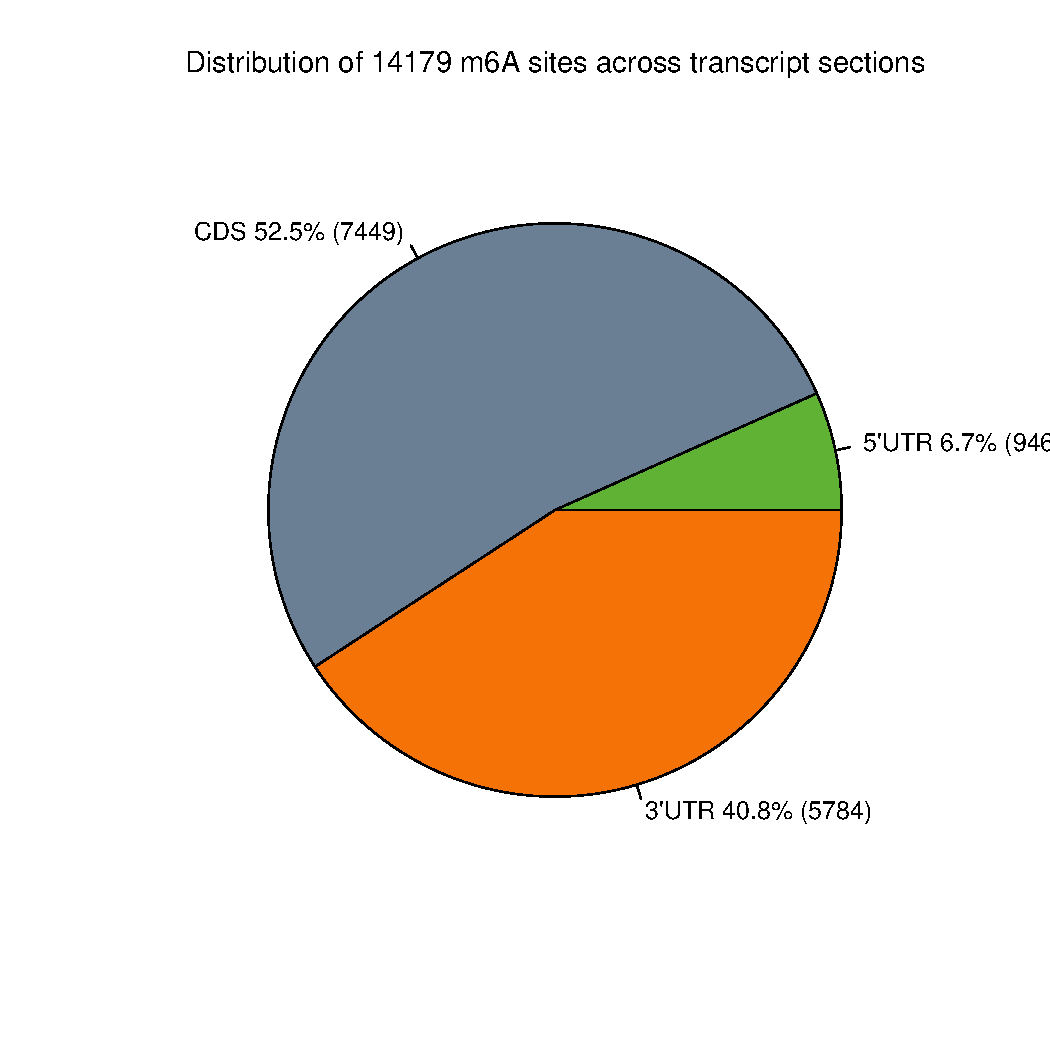
\includegraphics[width=\maxwidth]{figure/unnamed-chunk-7-1} 

\end{knitrout}
\end{document}
